\section{Phân tích yêu cầu}
\section{Thiết kế nền tảng}
\subsection{Thiết kế cơ chế truyền dữ liệu giữa Gateway và CoreIoT}

Trong hệ thống được xây dựng, Raspberry Pi 4 đóng vai trò gateway trung tâm, thực hiện chức năng thu thập dữ liệu từ các cảm biến, xử lý trạng thái hệ thống và truyền dữ liệu lên nền tảng quản lý IoT CoreIoT. Để đáp ứng yêu cầu truyền dữ liệu theo thời gian thực với mức tiêu thụ tài nguyên thấp, hệ thống sử dụng giao thức MQTT làm cơ chế giao tiếp chính giữa gateway và cloud server.

Gateway thực hiện kết nối đến MQTT Broker tại địa chỉ \texttt{App.\allowbreak coreiot.\allowbreak io} thông qua cổng \texttt{1883}. Quá trình xác thực sử dụng access token của thiết bị làm username cho phiên kết nối MQTT. Sau khi kết nối thành công, thiết bị định kỳ publish dữ liệu lên topic \texttt{v1/\allowbreak devices/\allowbreak me/\allowbreak telemetry} với chu kỳ 5 giây nhằm phục vụ việc giám sát và lưu trữ dữ liệu trên nền tảng cloud.

Dữ liệu được truyền lên hệ thống được đóng gói dưới dạng JSON nhằm đảm bảo tính linh hoạt và khả năng mở rộng trong quá trình xử lý phía server. Payload bao gồm các thông số môi trường được thu thập từ hệ thống cảm biến như nhiệt độ, độ ẩm, áp suất, cường độ ánh sáng và nồng độ bụi mịn PM2.5. Các giá trị này lần lượt được đọc từ các file trong hệ thống file của Linux như:

\begin{itemize}
    \item \texttt{/sys/class/sensorhub/hub0/temp}: dữ liệu nhiệt độ.
    \item \texttt{/sys/class/sensorhub/hub0/hum}: dữ liệu độ ẩm.
    \item \texttt{/sys/class/sensorhub/hub0/pressure}: dữ liệu áp suất môi trường.
    \item \texttt{/sys/class/sensorhub/hub0/lux}: dữ liệu cường độ ánh sáng.
    \item \texttt{/sys/class/sensorhub/hub0/pm25}: dữ liệu bụi mịn PM2.5.
\end{itemize}

Ngoài dữ liệu cảm biến thời gian thực, hệ thống còn tích hợp giá trị dự báo nồng độ PM2.5 trong 15 phút tiếp theo thông qua file tạm \texttt{/tmp/ai\_predict.txt}. Giá trị này được sử dụng nhằm hỗ trợ cơ chế cảnh báo sớm và nâng cao khả năng giám sát môi trường trong hệ thống kho thông minh.

Bên cạnh các thông số cảm biến, payload còn chứa các trường dữ liệu bổ trợ như mã thiết bị (\texttt{node}), chế độ hoạt động của hệ thống (\texttt{mode}) và timestamp thời gian thực được sinh từ hệ điều hành Linux thông qua hàm \texttt{time.time()}. Việc bổ sung timestamp giúp đảm bảo khả năng đồng bộ dữ liệu và hỗ trợ quá trình lưu trữ, truy vết dữ liệu trên nền tảng quản lý.

Trước khi dữ liệu được gửi lên MQTT Broker, gateway thực hiện một số bước tiền xử lý nhằm chuẩn hóa dữ liệu và xác định trạng thái hoạt động của hệ thống. Các giá trị cảm biến được đọc dưới dạng dữ liệu thô và được quy đổi sang giá trị thực tế thông qua các hệ số chia tương ứng. Trong đó, dữ liệu nhiệt độ được chia cho 10 để chuyển đổi sang đơn vị độ C, dữ liệu áp suất được chia cho 100 để đưa về đơn vị tiêu chuẩn, trong khi các thông số còn lại được giữ nguyên hoặc xử lý tùy theo đặc tính của từng cảm biến.

Sau giai đoạn tiền xử lý dữ liệu, gateway tiến hành đánh giá trạng thái vận hành của hệ thống dựa trên các ngưỡng cảnh báo đã được thiết lập trước. Quá trình đánh giá này nhằm xác định mức độ an toàn của môi trường kho và đưa ra cơ chế điều khiển phù hợp đối với quạt làm mát và relay.

Trong trường hợp nhiệt độ vượt quá 45\textdegree C hoặc giá trị dự báo PM2.5 lớn hơn 100, hệ thống sẽ lập tức chuyển sang trạng thái khẩn cấp \texttt{EMERGENCY\_FIRE}. Khi đó, quạt làm mát được kích hoạt ở mức cao nhất nhằm giảm thiểu nguy cơ mất an toàn trong môi trường vận hành.

Đối với điều kiện hoạt động thông thường, trạng thái hệ thống và mức điều khiển quạt được xác định dựa trên ngưỡng nhiệt độ như trình bày trong Bảng \ref{tab:system_state_logic}.

\begin{table}[H]
\centering
\begin{tabular}{|c|c|c|}
\hline
\textbf{Điều kiện} & \textbf{Trạng thái hệ thống} & \textbf{Mức quạt} \\ \hline
Nhiệt độ $<$ 30\textdegree C & NORMAL & LOW \\ \hline
30\textdegree C $\leq$ Nhiệt độ $<$ 40\textdegree C & WARNING & MEDIUM \\ \hline
Nhiệt độ $\geq$ 40\textdegree C & CRITICAL & HIGH \\ \hline
Nhiệt độ $>$ 45\textdegree C hoặc PM2.5 dự báo $>$ 100 & EMERGENCY\_FIRE & HIGH \\ \hline
\end{tabular}
\caption{Cơ chế xác định trạng thái hệ thống}
\label{tab:system_state_logic}
\end{table}

Bên cạnh cơ chế điều khiển theo ngưỡng nhiệt độ, hệ thống còn triển khai cơ chế giám sát trạng thái kéo dài nhằm phát hiện các tình huống bất thường trong quá trình vận hành. Nếu quạt duy trì ở mức \texttt{HIGH} liên tục trong hơn 30 giây, gateway sẽ chuyển hệ thống sang trạng thái \texttt{EMERGENCY\_SYSTEM}. Cơ chế này giúp nâng cao khả năng giám sát và tăng mức độ an toàn cho hệ thống trong môi trường thực tế.

Song song với quá trình điều khiển quạt, relay cũng được điều khiển tự động dựa trên nhiệt độ môi trường. Relay sẽ được kích hoạt khi nhiệt độ vượt quá 25\textdegree C và tự động tắt khi nhiệt độ giảm xuống dưới ngưỡng quy định.

Sau khi hoàn tất quá trình xử lý và đánh giá trạng thái, gateway tiến hành tổng hợp toàn bộ dữ liệu cảm biến và trạng thái hệ thống thành một payload hoàn chỉnh trước khi gửi lên nền tảng CoreIoT thông qua giao thức MQTT. Payload được xây dựng dưới dạng JSON nhằm đảm bảo khả năng mở rộng và dễ dàng tích hợp với hệ thống backend.

Cấu trúc dữ liệu được gửi lên hệ thống được mô tả trong Bảng \ref{tab:api_payload}.

\begin{table}[H]
\centering
\begin{tabular}{|c|l|l|}
\hline
\textbf{Trường dữ liệu} & \textbf{Ý nghĩa} & \textbf{Ví dụ} \\ \hline
\texttt{temperature} & Nhiệt độ môi trường & 32.5 \\ \hline
\texttt{humidity} & Độ ẩm môi trường & 75 \\ \hline
\texttt{light\_intensity} & Cường độ ánh sáng & 420 \\ \hline
\texttt{pm25} & Nồng độ bụi mịn PM2.5 & 18 \\ \hline
\texttt{stat} & Trạng thái hệ thống & WARNING \\ \hline
\texttt{node} & Mã thiết bị gateway & ESP\_01 \\ \hline
\texttt{mode} & Chế độ hoạt động & day \\ \hline
\texttt{timestamp} & Thời gian gửi dữ liệu & 1715259000 \\ \hline
\end{tabular}
\caption{Cấu trúc payload dữ liệu gửi lên CoreIoT}
\label{tab:api_payload}
\end{table}

Từ cấu trúc trên, payload JSON được gửi lên MQTT Broker có dạng như sau:

\begin{verbatim}
{
    "temperature": 32.5,
    "humidity": 75,
    "light_intensity": 420,
    "pm25": 18,
    "stat": "WARNING",
    "node": "ESP_01",
    "mode": "day",
    "timestamp": "1715259000"
}
\end{verbatim}

Toàn bộ quá trình từ thu thập dữ liệu cảm biến, xử lý trạng thái hệ thống, xây dựng payload đến publish dữ liệu lên CoreIoT được thực hiện liên tục theo chu kỳ 5 giây thông qua vòng lặp chính của chương trình gateway. Để đảm bảo tính ổn định của hệ thống, các lỗi phát sinh trong quá trình đọc dữ liệu cảm biến hoặc truy xuất file dự báo AI đều được xử lý bằng cơ chế fallback, trong đó giá trị mặc định được gán bằng 0 nhằm tránh gián đoạn luồng dữ liệu gửi lên hệ thống cloud.
Quá trình thu thập dữ liệu, xử lý logic và truyền dữ liệu được thực hiện liên tục theo chu kỳ 5 giây thông qua vòng lặp chính của chương trình gateway. Để đảm bảo tính ổn định của hệ thống, các lỗi phát sinh trong quá trình đọc dữ liệu cảm biến hoặc truy xuất file dự báo AI đều được xử lý bằng cơ chế fallback, trong đó giá trị mặc định được gán bằng 0 nhằm tránh gián đoạn luồng dữ liệu gửi lên hệ thống cloud.

\begin{figure}[!h]
    \centering
    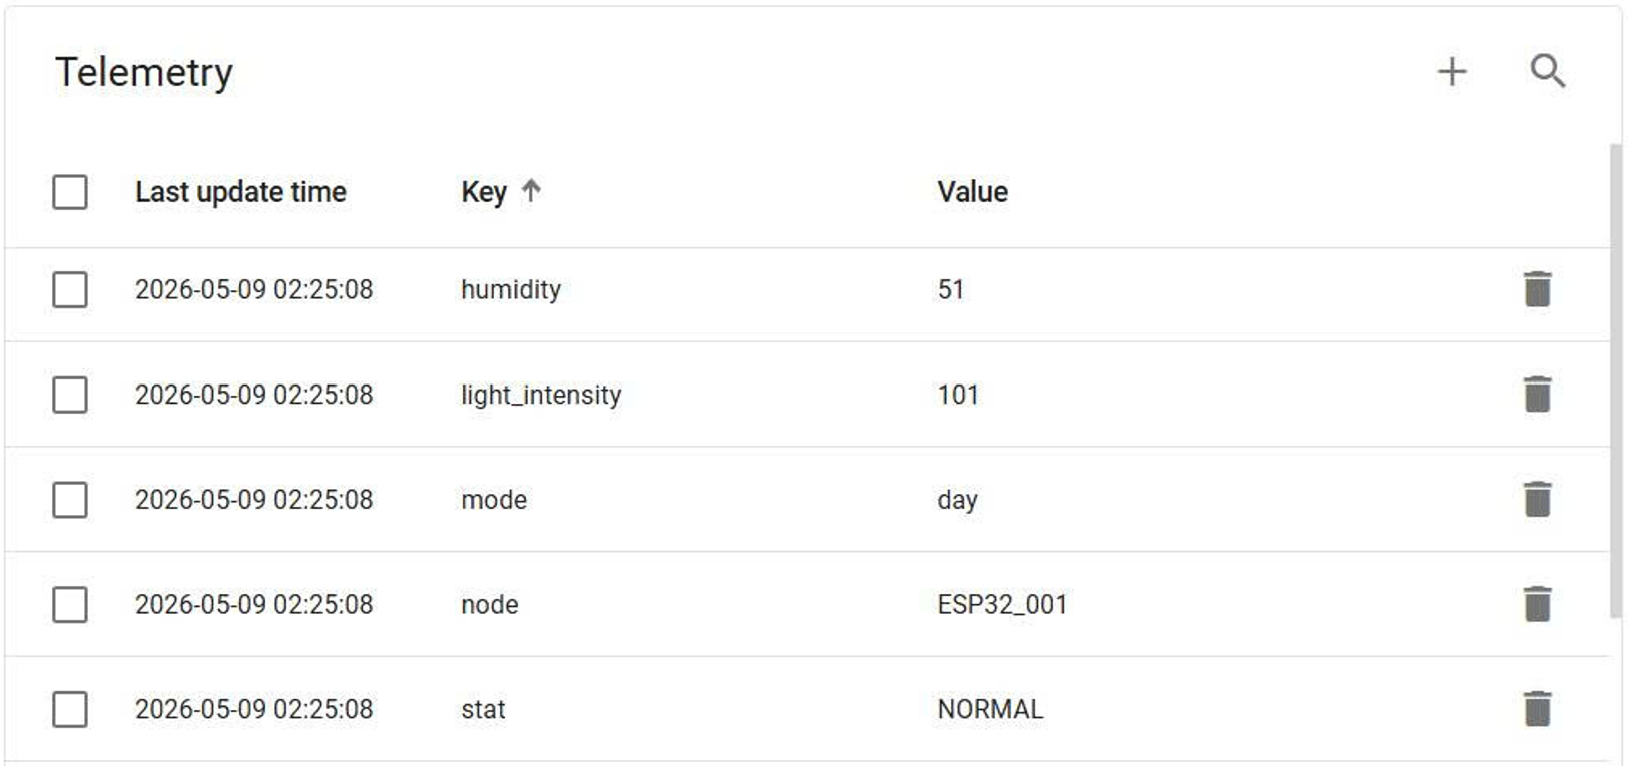
\includegraphics[width=1\textwidth]{image/api.png}
    \caption{Định dạng dữ liệu được gửi lên CoreIot}
    \label{fig:rulechain}
\end{figure}
\newpage

\section{Thiết kế khối xử lý}
\subsection{Khối xử lý cảnh báo}

Hình \ref{fig:warning_block} mô tả kiến trúc tổng thể của khối xử lý cảnh báo được triển khai trên nền tảng gateway sử dụng Raspberry Pi 4. Khối chức năng này có nhiệm vụ thu thập dữ liệu cảm biến, tiền xử lý dữ liệu, thực hiện phân tích bằng Rule Chain kết hợp AI, sau đó đưa ra mức cảnh báo phù hợp để hiển thị trên các giao diện giám sát.

\begin{figure}[H]
    \centering
    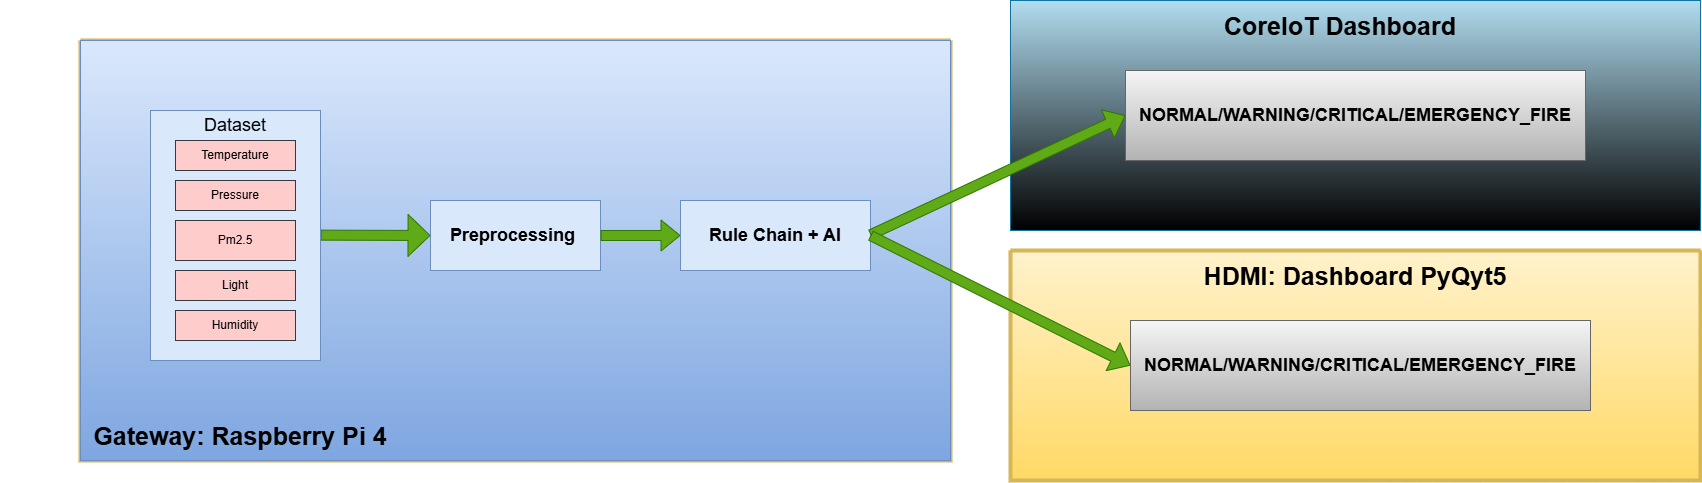
\includegraphics[width=0.95\linewidth]{image/warnblock.png}
    \caption{Kiến trúc khối xử lý cảnh báo trên gateway Raspberry Pi 4}
    \label{fig:warning_block}
\end{figure}

Trong hệ thống, các dữ liệu đầu vào bao gồm nhiệt độ (Temperature), áp suất (Pressure), bụi mịn PM2.5, cường độ ánh sáng (Light) và độ ẩm (Humidity). Các dữ liệu này được thu thập từ cảm biến thông qua các giao thức truyền thông như I2C và Modbus RTU RS485, sau đó được đưa vào gateway Raspberry Pi 4 để xử lý.

Sau khi tiếp nhận dữ liệu, hệ thống thực hiện bước \textbf{Preprocessing} nhằm chuẩn hóa dữ liệu đầu vào, loại bỏ nhiễu, kiểm tra giá trị bất thường và chuyển đổi dữ liệu về định dạng phù hợp cho quá trình phân tích. Đây là bước quan trọng giúp tăng độ ổn định và độ chính xác của hệ thống cảnh báo.

Tiếp theo, dữ liệu được đưa vào khối \textbf{Rule Chain + AI}. Tại đây, hệ thống áp dụng tập luật (Rule Chain) kết hợp với thuật toán AI nhằm đánh giá trạng thái môi trường theo thời gian thực. Các luật được xây dựng dựa trên ngưỡng an toàn của từng loại cảm biến, đồng thời AI hỗ trợ phân tích xu hướng và nhận diện các trạng thái nguy hiểm phức tạp hơn.

Kết quả phân tích sẽ được phân loại thành các mức cảnh báo gồm:

\begin{itemize}
    \item \textbf{NORMAL}: Trạng thái hoạt động bình thường.
    \item \textbf{WARNING}: Có dấu hiệu bất thường nhẹ, cần theo dõi.
    \item \textbf{CRITICAL}: Mức nguy hiểm cao, cần xử lý kịp thời.
    \item \textbf{EMERGENCY\_FIRE}: Phát hiện nguy cơ cháy hoặc sự cố nghiêm trọng.
\end{itemize}

Các trạng thái cảnh báo sau khi được xác định sẽ được đồng bộ và hiển thị trên hai nền tảng:

\begin{itemize}
    \item \textbf{CoreIoT Dashboard}: Dashboard giám sát từ xa thông qua nền tảng IoT.
    \item \textbf{HDMI Dashboard PyQt5}: Dashboard cục bộ hiển thị trực tiếp trên màn hình HDMI kết nối với Raspberry Pi 4.
\end{itemize}

Việc triển khai song song hai cơ chế hiển thị giúp hệ thống đảm bảo khả năng giám sát linh hoạt, vừa hỗ trợ quản lý tập trung từ xa, vừa cho phép theo dõi trực tiếp tại thiết bị gateway. Đồng thời, kiến trúc xử lý tại biên (Edge Computing) giúp giảm độ trễ phản hồi, hạn chế phụ thuộc vào kết nối Internet và tăng khả năng hoạt động ổn định trong các môi trường tự động hóa công nghiệp.

\section{Thiết kế giao diện người dùng}


